\sectionframe{What a time series is}{Order, seasonality, drift, gaps and company}

\begin{frame}{A time series is a set of values indexed by time, and the order carries the information}
  A series $y_1, \dots, y_T$ is sampled at a fixed frequency, here one count per hour.
  \begin{center}
    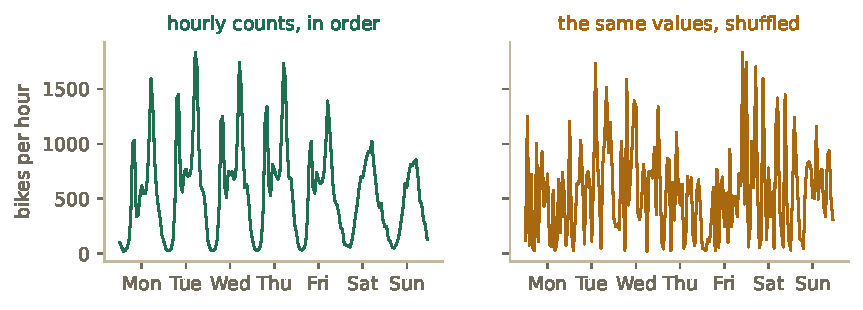
\includegraphics[width=.75\textwidth]{week_shuffled}
  \end{center}
  Shuffling the rows of a table loses nothing. Shuffling a series destroys it.
  \takeaway{Models must use the order: what came before predicts what comes next.}
\end{frame}

\begin{frame}{Time series are everywhere, at every scale of time}
  \begin{center}
    \renewcommand{\arraystretch}{1.15}
    \begin{tabular}{lll}
      \toprule
      \head{Series} & \head{Sampling} & \head{Example} \\
      \midrule
      EEG & 1 ms & sleep stages, brain-computer interfaces \\
      Electricity load & 15 min & grid balancing \\
      Bike counts & 1 hour & the Paris counters of this tutorial \\
      Retail sales & 1 day & stock planning \\
      Atmospheric CO$_2$ & 1 month & Mauna Loa since 1958 \\
      Variable stars & irregular & light curves of telescopes \\
      \bottomrule
    \end{tabular}
  \end{center}
  \takeaway{Sampling frequencies span about ten orders of magnitude.}
\end{frame}

\begin{frame}{Real series stack several seasonalities on top of a trend}
  \begin{center}
    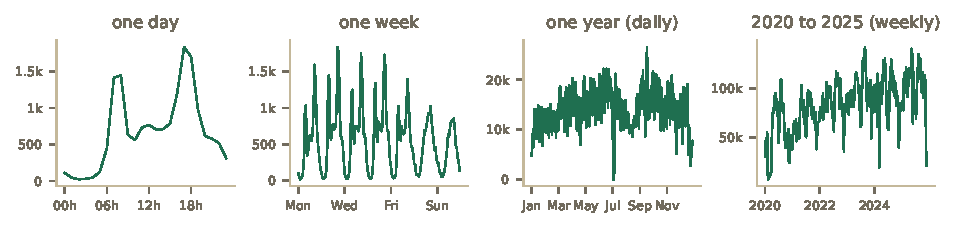
\includegraphics[width=\textwidth]{seasonalities}
  \end{center}
  Boulevard de Sébastopol, both directions: a daily cycle with two commute peaks,
  a weekly cycle, a yearly cycle, and a trend that changes with the city.
  \takeaway{The structure lives at several time scales at once.}
\end{frame}

\begin{frame}{Real series are not stationary}
  \begin{columns}[c]
    \column{.62\textwidth}
    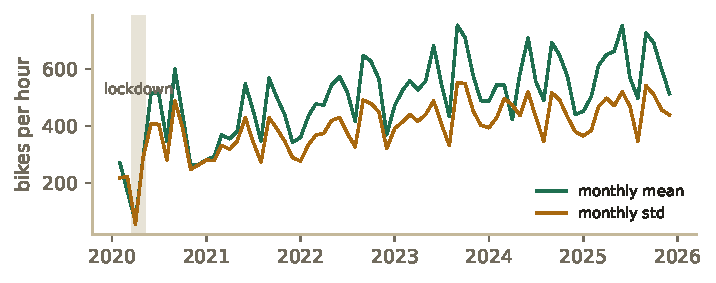
\includegraphics[width=\textwidth]{nonstationary}
    \column{.34\textwidth}
    \begin{itemize}
      \item Level shifts: lockdowns, new bike lanes.
      \item The variance grows with the level.
      \item Holidays and strikes break the weekly pattern.
    \end{itemize}
  \end{columns}
  \takeaway{The past is a guide to the future, not a copy of it.}
\end{frame}

\begin{frame}{Real series are messy: gaps, outliers and counting artefacts}
  \begin{center}
    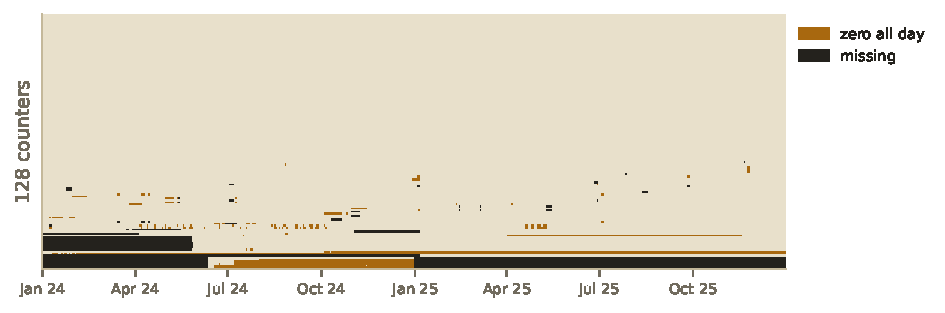
\includegraphics[width=.9\textwidth]{missing_2025}
  \end{center}
  Counters go offline for weeks, broken sensors report zeros, and the clock change
  makes days of 23 or 25 hours.
  \takeaway{Cleaning and checking the data comes before any model.}
\end{frame}

\begin{frame}{A series rarely comes alone}
  \begin{columns}[T]
    \column{.31\textwidth}
    \begin{block}{Channels}
      Several measures of one system: both directions of a counter, the electrodes of an EEG.
    \end{block}
    \column{.31\textwidth}
    \begin{alertblock}{Covariates}
      Variables that drive the target: weather, holidays, prices.
    \end{alertblock}
    \column{.31\textwidth}
    \begin{exampleblock}{Related series}
      Many series of the same kind: every bike counter of Paris.
    \end{exampleblock}
  \end{columns}
  \takeaway{Using what comes with the target is where the gains are.}
\end{frame}

\begin{frame}{Covariates differ by what we know when we forecast}
  \begin{center}
    \begin{tikzpicture}[x=1cm, y=.75cm, font=\small]
      \fill[tmtint] (0, -.4) rectangle (7, 3.4);
      \draw[tmmuted, thick] (7, -.6) -- (7, 3.7) node[above, font=\scriptsize\bfseries, text=tmaccent] {forecast origin};
      \node[tmmuted, font=\scriptsize] at (3.5, -.8) {past (context)};
      \node[tmmuted, font=\scriptsize] at (10, -.8) {future (horizon)};
      \foreach \y/\name/\stop/\col in {3/{static: location of the counter}/13/tmprimary,
                                       2/{known in the future: calendar, holidays}/13/tmprimary,
                                       1/{past only: observed weather}/7/tmaccent,
                                       0/{target: bike counts}/7/tmink} {
        \draw[\col, line width=2pt] (0, \y) -- (\stop, \y);
        \node[anchor=west, font=\scriptsize, text=\col, fill=tmpaper, inner sep=1pt] at (.2, \y+.35) {\name};
      }
    \end{tikzpicture}
  \end{center}
  A weather forecast turns past-only weather into a known-future covariate, with errors.
  \takeaway{This vocabulary returns in the tour of design decisions.}
\end{frame}
